\documentclass[11pt]{article}

% ---- packages just for THIS guide (not related to your paper) ----
\usepackage[margin=1in]{geometry}
\usepackage{parskip}          % blank line between paragraphs, no indent
\usepackage{xcolor}
\usepackage{listings}         % for showing code in boxes
\usepackage{enumitem}
\usepackage{titlesec}
\usepackage[hidelinks]{hyperref}

\definecolor{codebg}{RGB}{245,246,248}
\definecolor{codeframe}{RGB}{210,214,220}
\definecolor{accent}{RGB}{20,80,140}

\titleformat{\section}{\Large\bfseries\color{accent}}{\thesection.}{0.5em}{}
\titleformat{\subsection}{\large\bfseries}{\thesubsection}{0.5em}{}

% style for the code boxes
\lstset{
  basicstyle=\ttfamily\small,
  backgroundcolor=\color{codebg},
  frame=single,
  rulecolor=\color{codeframe},
  framesep=6pt,
  breaklines=true,
  breakatwhitespace=false,
  columns=fullflexible,
  keepspaces=true,
  showstringspaces=false,
  xleftmargin=4pt,
  aboveskip=8pt,
  belowskip=8pt,
}

% a small command for "inline code": use \code{...}
% (we mostly use \verb for things with backslashes)
\newcommand{\code}[1]{\texttt{#1}}

\title{\vspace{-1.5cm}\textbf{Understanding the LaTeX in \texttt{main.tex}}\\[2mm]
\large A beginner's walkthrough of every command used in the NanoFlow report}
\author{}
\date{}

\begin{document}
\maketitle
\vspace{-1cm}

This guide explains the LaTeX ``syntax'' (the commands) that appear in your
\verb|main.tex| file, grouped by topic. For each one you get: what it looks like
in your file, and what it actually does. Nothing here changes your paper --- it is
just a reference so you can explain the file confidently.

A quick mental model first: \textbf{a LaTeX command almost always starts with a
backslash} (\verb|\|), like \verb|\section| or \verb|\textbf|. Many commands take
an \emph{argument} in curly braces \verb|{ }|, and some take \emph{options} in
square brackets \verb|[ ]|. So \verb|\command[option]{argument}| is the general
shape. Anything after a percent sign \verb|%| on a line is a \textbf{comment} ---
LaTeX ignores it, so it is just a note to yourself.

\tableofcontents

% ======================================================================
\section{How the whole document is put together}

Every LaTeX file has two parts:

\begin{enumerate}[leftmargin=*]
  \item The \textbf{preamble} --- everything from the top of the file down to
        \verb|\begin{document}|. This is \emph{setup}: which document style to
        use, which add-on packages to load, and any custom shortcuts. Nothing here
        prints directly.
  \item The \textbf{body} --- everything between \verb|\begin{document}| and
        \verb|\end{document}|. This is the actual content that becomes pages.
\end{enumerate}

\begin{lstlisting}
\documentclass[manuscript,review]{acmart}   % preamble starts here
...packages and settings...
\begin{document}
...your paper...
\end{document}
\end{lstlisting}

\textbf{Environments.} Whenever you see a matching pair
\verb|\begin{something}| \dots \verb|\end{something}|, that is called an
\emph{environment}. The \verb|document| environment above is the biggest one;
later you will see \verb|abstract|, \verb|figure|, \verb|table|, \verb|tabular|,
\verb|itemize|, \verb|equation|, and \verb|algorithm| environments.

\textbf{How a PDF is produced.} The \verb|.tex| file is \emph{compiled} into a
PDF. Because the paper has citations and cross-references, the tool has to run a
few times: LaTeX runs once, then \verb|bibtex| builds the reference list from the
\verb|.bib| file, then LaTeX runs a couple more times so all the ``Figure~3'' and
``[12]'' numbers settle. The \verb|latexmk| tool just does all of that for you in
one command.

% ======================================================================
\section{The document class and packages}

\subsection{\texttt{\textbackslash documentclass}}

\begin{lstlisting}
\documentclass[manuscript,review]{acmart}
\end{lstlisting}

This is always the very first line. It chooses the overall \emph{style} of the
document. Here the class is \verb|acmart| (the official style of the ACM, the
Association for Computing Machinery --- the publisher your source paper uses). The
words in brackets, \verb|manuscript| and \verb|review|, are \emph{options} that
tell \verb|acmart| to use the single-column, larger-font ``manuscript'' layout
with ``review'' spacing. Your assignment specifically required this exact line.

\subsection{\texttt{\textbackslash usepackage} --- loading add-ons}

LaTeX by itself is fairly basic; \textbf{packages} add features. You load one with
\verb|\usepackage{name}|. Here is every package in your file and why it is there:

\begin{lstlisting}
\usepackage{graphicx}      % lets you insert images (\includegraphics)
\usepackage{booktabs}      % nicer horizontal lines in tables
\usepackage{amsmath}       % proper math typesetting (equations, \frac, ...)
\usepackage{amssymb}       % extra math symbols
\usepackage{xspace}        % smart spacing after your custom \nf command
\usepackage{multirow}      % lets a table cell span several rows
\usepackage{algorithm}     % the floating "Algorithm 1" box
\usepackage{algpseudocode} % the pseudocode commands (\State, \For, ...)
\usepackage{tikz}          % a drawing package (loaded, available if needed)
\end{lstlisting}

The line right after loads a \verb|tikz| ``library'' (an add-on for the drawing
package):

\begin{lstlisting}
\usetikzlibrary{shapes.geometric, arrows.meta, positioning, calc, fit, backgrounds}
\end{lstlisting}

\subsection{\texttt{\textbackslash graphicspath}}

\begin{lstlisting}
\graphicspath{{figures/}}
\end{lstlisting}

This tells LaTeX ``look inside the \verb|figures/| folder for images.'' That is
why later you can write \verb|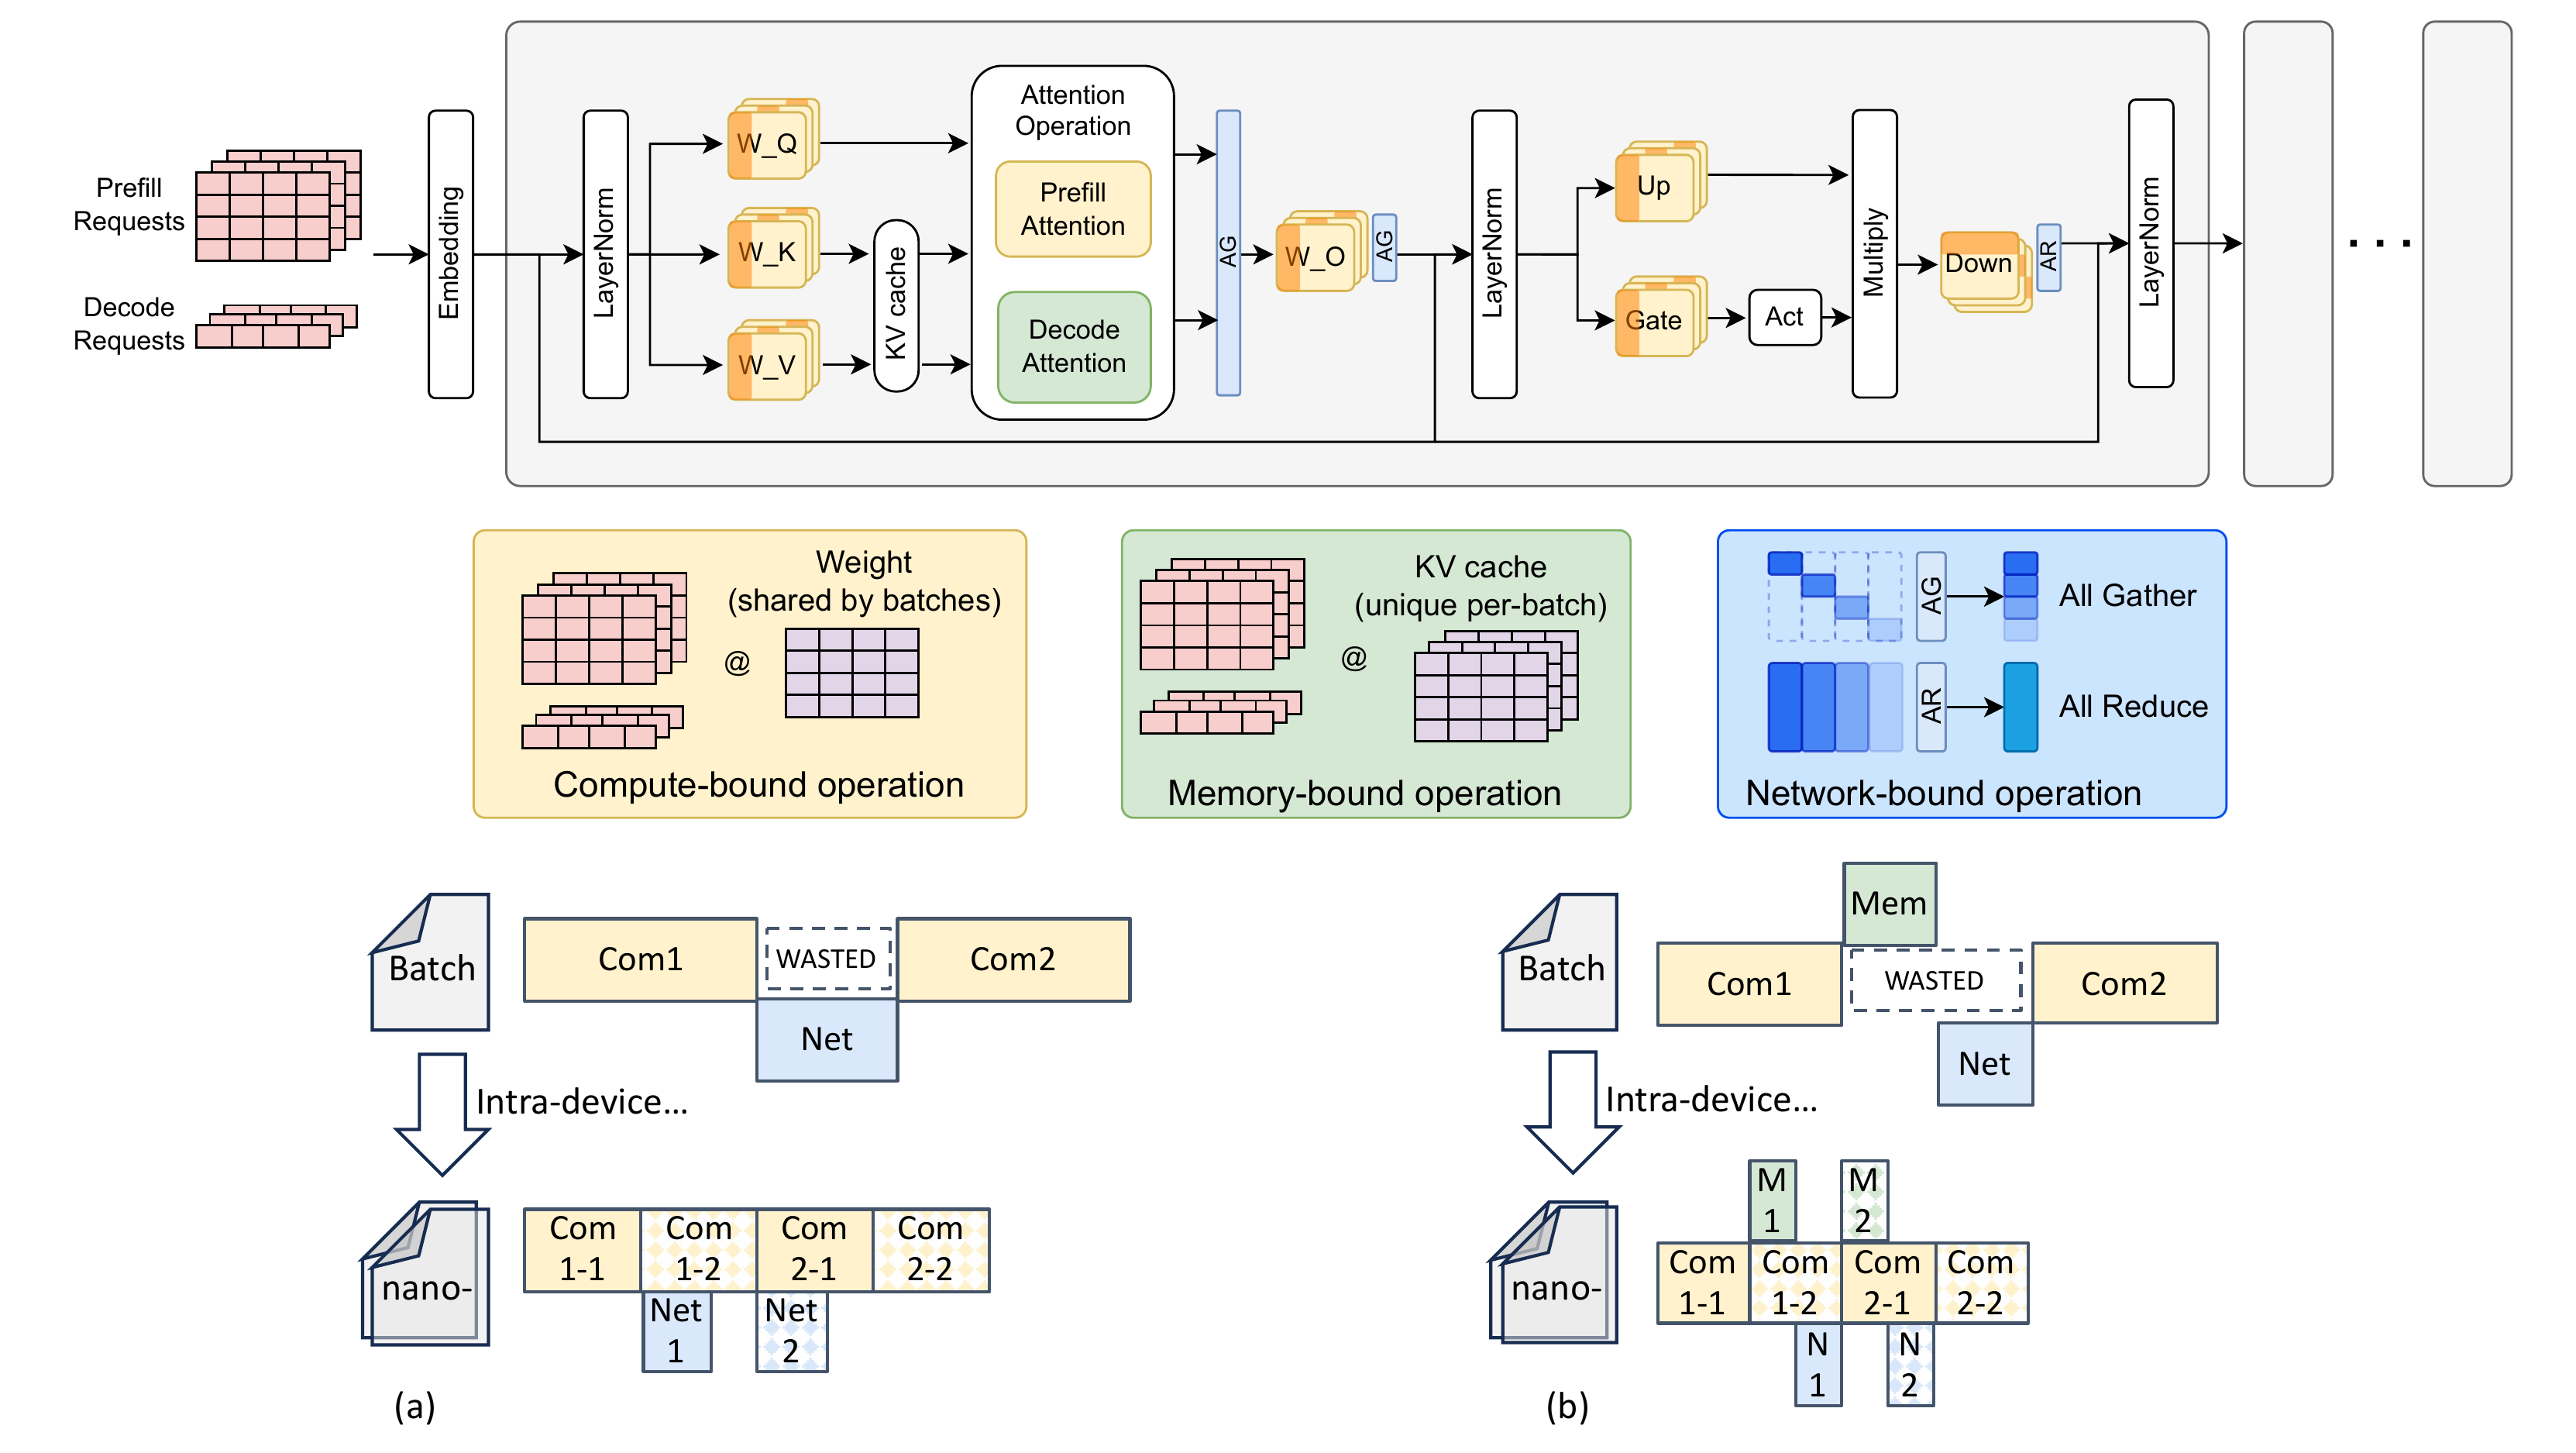
\includegraphics{fig1_transformer.png}| without
typing the folder name every time.

% ======================================================================
\section{Preamble settings and custom shortcuts}

\subsection{Turning off ACM boilerplate}

Because your paper is a class reproduction, not a real ACM submission, a few lines
switch off the copyright notice and reference block that \verb|acmart| would
normally force:

\begin{lstlisting}
\settopmatter{printacmref=false}                 % no "ACM Reference Format" block
\renewcommand\footnotetextcopyrightpermission[1]{} % blank out the copyright footnote
\pagestyle{plain}                                % simple page numbers
\setcopyright{none}                              % no copyright statement
\acmConference[Reproduction Report]{CSE 200: ...}{...}{...}
\acmYear{2026}
\copyrightyear{2026}
\end{lstlisting}

The \verb|\acmConference|, \verb|\acmYear|, and \verb|\copyrightyear| lines just
fill in the venue/date fields that \verb|acmart| expects.

\subsection{\texttt{\textbackslash newcommand} --- making your own shortcut}

\begin{lstlisting}
\newcommand{\nf}{\textsc{NanoFlow}\xspace}
\end{lstlisting}

This \emph{defines a new command}. After this line, every time you type
\verb|\nf| in the paper, LaTeX replaces it with \verb|\textsc{NanoFlow}| (which
prints ``\textsc{NanoFlow}'' in small capitals). This is handy because the name
appears dozens of times --- if you ever wanted to restyle it, you would change one
line instead of hundreds. The \verb|\xspace| at the end politely adds a space
after the word when one is needed (so ``\nf runs'' does not become ``NanoFlowruns'')
but not before punctuation.

The next three define math shortcuts the same way:

\begin{lstlisting}
\newcommand{\Bdense}{B_{\mathit{Dense}}}   % prints B with subscript "Dense"
\newcommand{\Pmodel}{P_{\mathit{Model}}}
\newcommand{\Dmodel}{D_{\mathit{model}}}
\end{lstlisting}

Here \verb|_| means ``subscript'' and \verb|\mathit{...}| makes the subscript word
italic. So \verb|\Bdense| is a shortcut for the symbol $B_{Dense}$.

\subsection{\texttt{\textbackslash renewcommand} and \texttt{\textbackslash let}}

\verb|\newcommand| makes a \emph{new} command; \verb|\renewcommand| \emph{changes
an existing} one. You use it here to set the short author name shown in page
headers:

\begin{lstlisting}
\renewcommand{\shortauthors}{Zhu et al.}
\end{lstlisting}

\verb|\let| is a lower-level ``copy this meaning'' command. We used it once as a
fix (explained in Section~\ref{sec:fixes}).

% ======================================================================
\section{The title block (authors, abstract, title)}

Everything that makes the ``header'' of the paper sits between
\verb|\begin{document}| and \verb|\maketitle|.

\begin{lstlisting}
\title{NanoFlow: Towards Optimal Large Language Model Serving Throughput}

\author{Kan Zhu}
\affiliation{%
  \institution{University of Washington}
  \country{USA}
}
\end{lstlisting}

\begin{itemize}[leftmargin=*]
  \item \verb|\title{...}| sets the paper title.
  \item \verb|\author{...}| names one author. You repeat this block for each of
        the 17 authors.
  \item \verb|\affiliation{...}| holds that author's institution info.
  \item \verb|\institution{...}| and \verb|\country{...}| go \emph{inside}
        \verb|\affiliation|. The \verb|acmart| class \textbf{requires} a country,
        which is why every block has \verb|\country{USA}| (that was one of the
        errors we fixed early on).
  \item The lone \verb|%| right after \verb|\affiliation{| is a trick: it hides
        the line break so no stray space sneaks in. A comment ``eats'' the
        newline.
\end{itemize}

Then the abstract and keywords:

\begin{lstlisting}
\begin{abstract}
Large Language Models (LLMs) have resulted in ...
\end{abstract}

\keywords{Large Language Models, Inference Serving, ...}

\maketitle
\end{lstlisting}

\verb|abstract| is an environment holding the summary paragraph.
\verb|\keywords{...}| lists the topic tags. Finally \verb|\maketitle| is the
command that actually \emph{draws} the title, authors, and abstract onto the page
using all the info above. Nothing appears until \verb|\maketitle| is called.

% ======================================================================
\section{Section headings and cross-references}

\subsection{Headings}

\begin{lstlisting}
\section{Introduction}
\subsection{The LLM Inference Workflow}
\subsubsection{Parameters}
\end{lstlisting}

These create numbered headings at three levels (1, 1.1, 1.1.1). LaTeX numbers
them automatically --- if you reorder sections, the numbers update themselves.

\subsection{Labels and references}

\begin{lstlisting}
\section{Method}
\label{sec:method}
...
... discussed in Section~\ref{sec:method}.
\end{lstlisting}

\verb|\label{name}| puts an invisible ``bookmark'' on the thing just before it (a
section, figure, table, or equation). \verb|\ref{name}| then prints that thing's
\emph{number} wherever you mention it. So if Method is section 3, \verb|\ref| prints
``3''. This is why the report can say ``see Section~\ref{sec:results}'' and always
get the right number, even after edits. The names like \verb|sec:method|,
\verb|fig:transformer|, \verb|tab:datasets|, \verb|eq:optimal| are just labels you
choose; the \verb|sec:|/\verb|fig:|/\verb|tab:|/\verb|eq:| prefixes are a common
habit to keep them organized.

\subsection{Citations and the \texttt{\~{}} symbol}

\begin{lstlisting}
... office suites~\cite{mehdi2023bing, openai2023chatgpt, spataro2023copilot}.
\end{lstlisting}

\verb|\cite{key}| prints a reference number like ``[5]'' and adds that source to
the reference list. The \verb|key| (e.g.\ \verb|mehdi2023bing|) must match an
entry in your \verb|references.bib| file. You can cite several at once separated
by commas.

The \verb|~| (tilde) before \verb|\cite| is a \textbf{non-breaking space}: a space
that will never be split across a line break. It keeps the word and its citation
number together, so you never get ``suites'' at the end of one line and ``[5]''
alone at the start of the next. You will see \verb|~| used before \verb|\ref| and
\verb|\cite| throughout.

% ======================================================================
\section{Formatting text and special characters}

\subsection{Font styles}

\begin{lstlisting}
\textbf{Dense operations.}   % bold
\emph{compute-bound}         % emphasis (usually italic)
\textsc{NanoFlow}            % SMALL CAPS
\texttt{max-num-tokens}      % typewriter / monospace font
\end{lstlisting}

\subsection{Characters that need special handling}

Some characters have special meaning in LaTeX, so to \emph{print} them you escape
them with a backslash:

\begin{lstlisting}
50\%        % a literal percent sign  (bare % would start a comment!)
72\%        % same
prefill \& decode   % a literal & (bare & is a table column separator)
\end{lstlisting}

Other useful bits you will see:

\begin{itemize}[leftmargin=*]
  \item \verb|---| becomes a long ``em dash'' (---), used for breaks in a
        sentence. (\verb|--| is a medium dash for ranges, like 50--72\%.)
  \item Quotes are written with backticks and apostrophes:
        \verb|``WASTED''| prints proper curly quotes ``WASTED''.
  \item \verb|\,| inserts a \emph{thin space}, used in numbers with units like
        \verb|80\,GB| or \verb|200\,ms| so the number and unit sit close but not
        touching.
  \item \verb|\S| prints the section symbol (\S), as in \verb|\S\ref{sec:runtime}|.
\end{itemize}

% ======================================================================
\section{Math and equations}

\subsection{Inline math}

Anything between two dollar signs is typeset as math:

\begin{lstlisting}
Mixtral 8$\times$7B          % the $\times$ prints a multiplication sign
$T_R < 1$ means compute-bound.
$1 \ldots t{-}1$             % \ldots is "...", {-} keeps the minus tidy
\end{lstlisting}

\subsection{Displayed, numbered equations}

\begin{lstlisting}
\begin{equation}
  T_{mem} = \frac{MemSize}{MemBW}.
  \label{eq:tmem}
\end{equation}
\end{lstlisting}

The \verb|equation| environment puts the formula on its own centered line and
gives it a number (which you can point at with \verb|\ref{eq:tmem}|). Common
pieces inside:

\begin{itemize}[leftmargin=*]
  \item \verb|\frac{top}{bottom}| makes a fraction.
  \item \verb|_| is subscript and \verb|^| is superscript
        (e.g.\ \verb|\Dmodel^2| is $D^2$, \verb|10^{-5}| is $10^{-5}$).
  \item \verb|\approx|, \verb|\le|, \verb|\times|, \verb|\cdot| print
        $\approx$, $\le$, $\times$, $\cdot$.
  \item \verb|\mathit{Dense}| writes a whole word in math italic.
\end{itemize}

% ======================================================================
\section{Bulleted lists}

\begin{lstlisting}
\begin{itemize}
  \item An analytical cost model ...
  \item \nf: an MILP auto-search engine ...
  \item An evaluation showing 1.91$\times$ throughput ...
\end{itemize}
\end{lstlisting}

\verb|itemize| makes a bulleted list; each bullet starts with \verb|\item|.
(A numbered list would use \verb|enumerate| instead.)

% ======================================================================
\section{Figures (inserting images)}

\begin{lstlisting}
\begin{figure}[t]
  \centering
  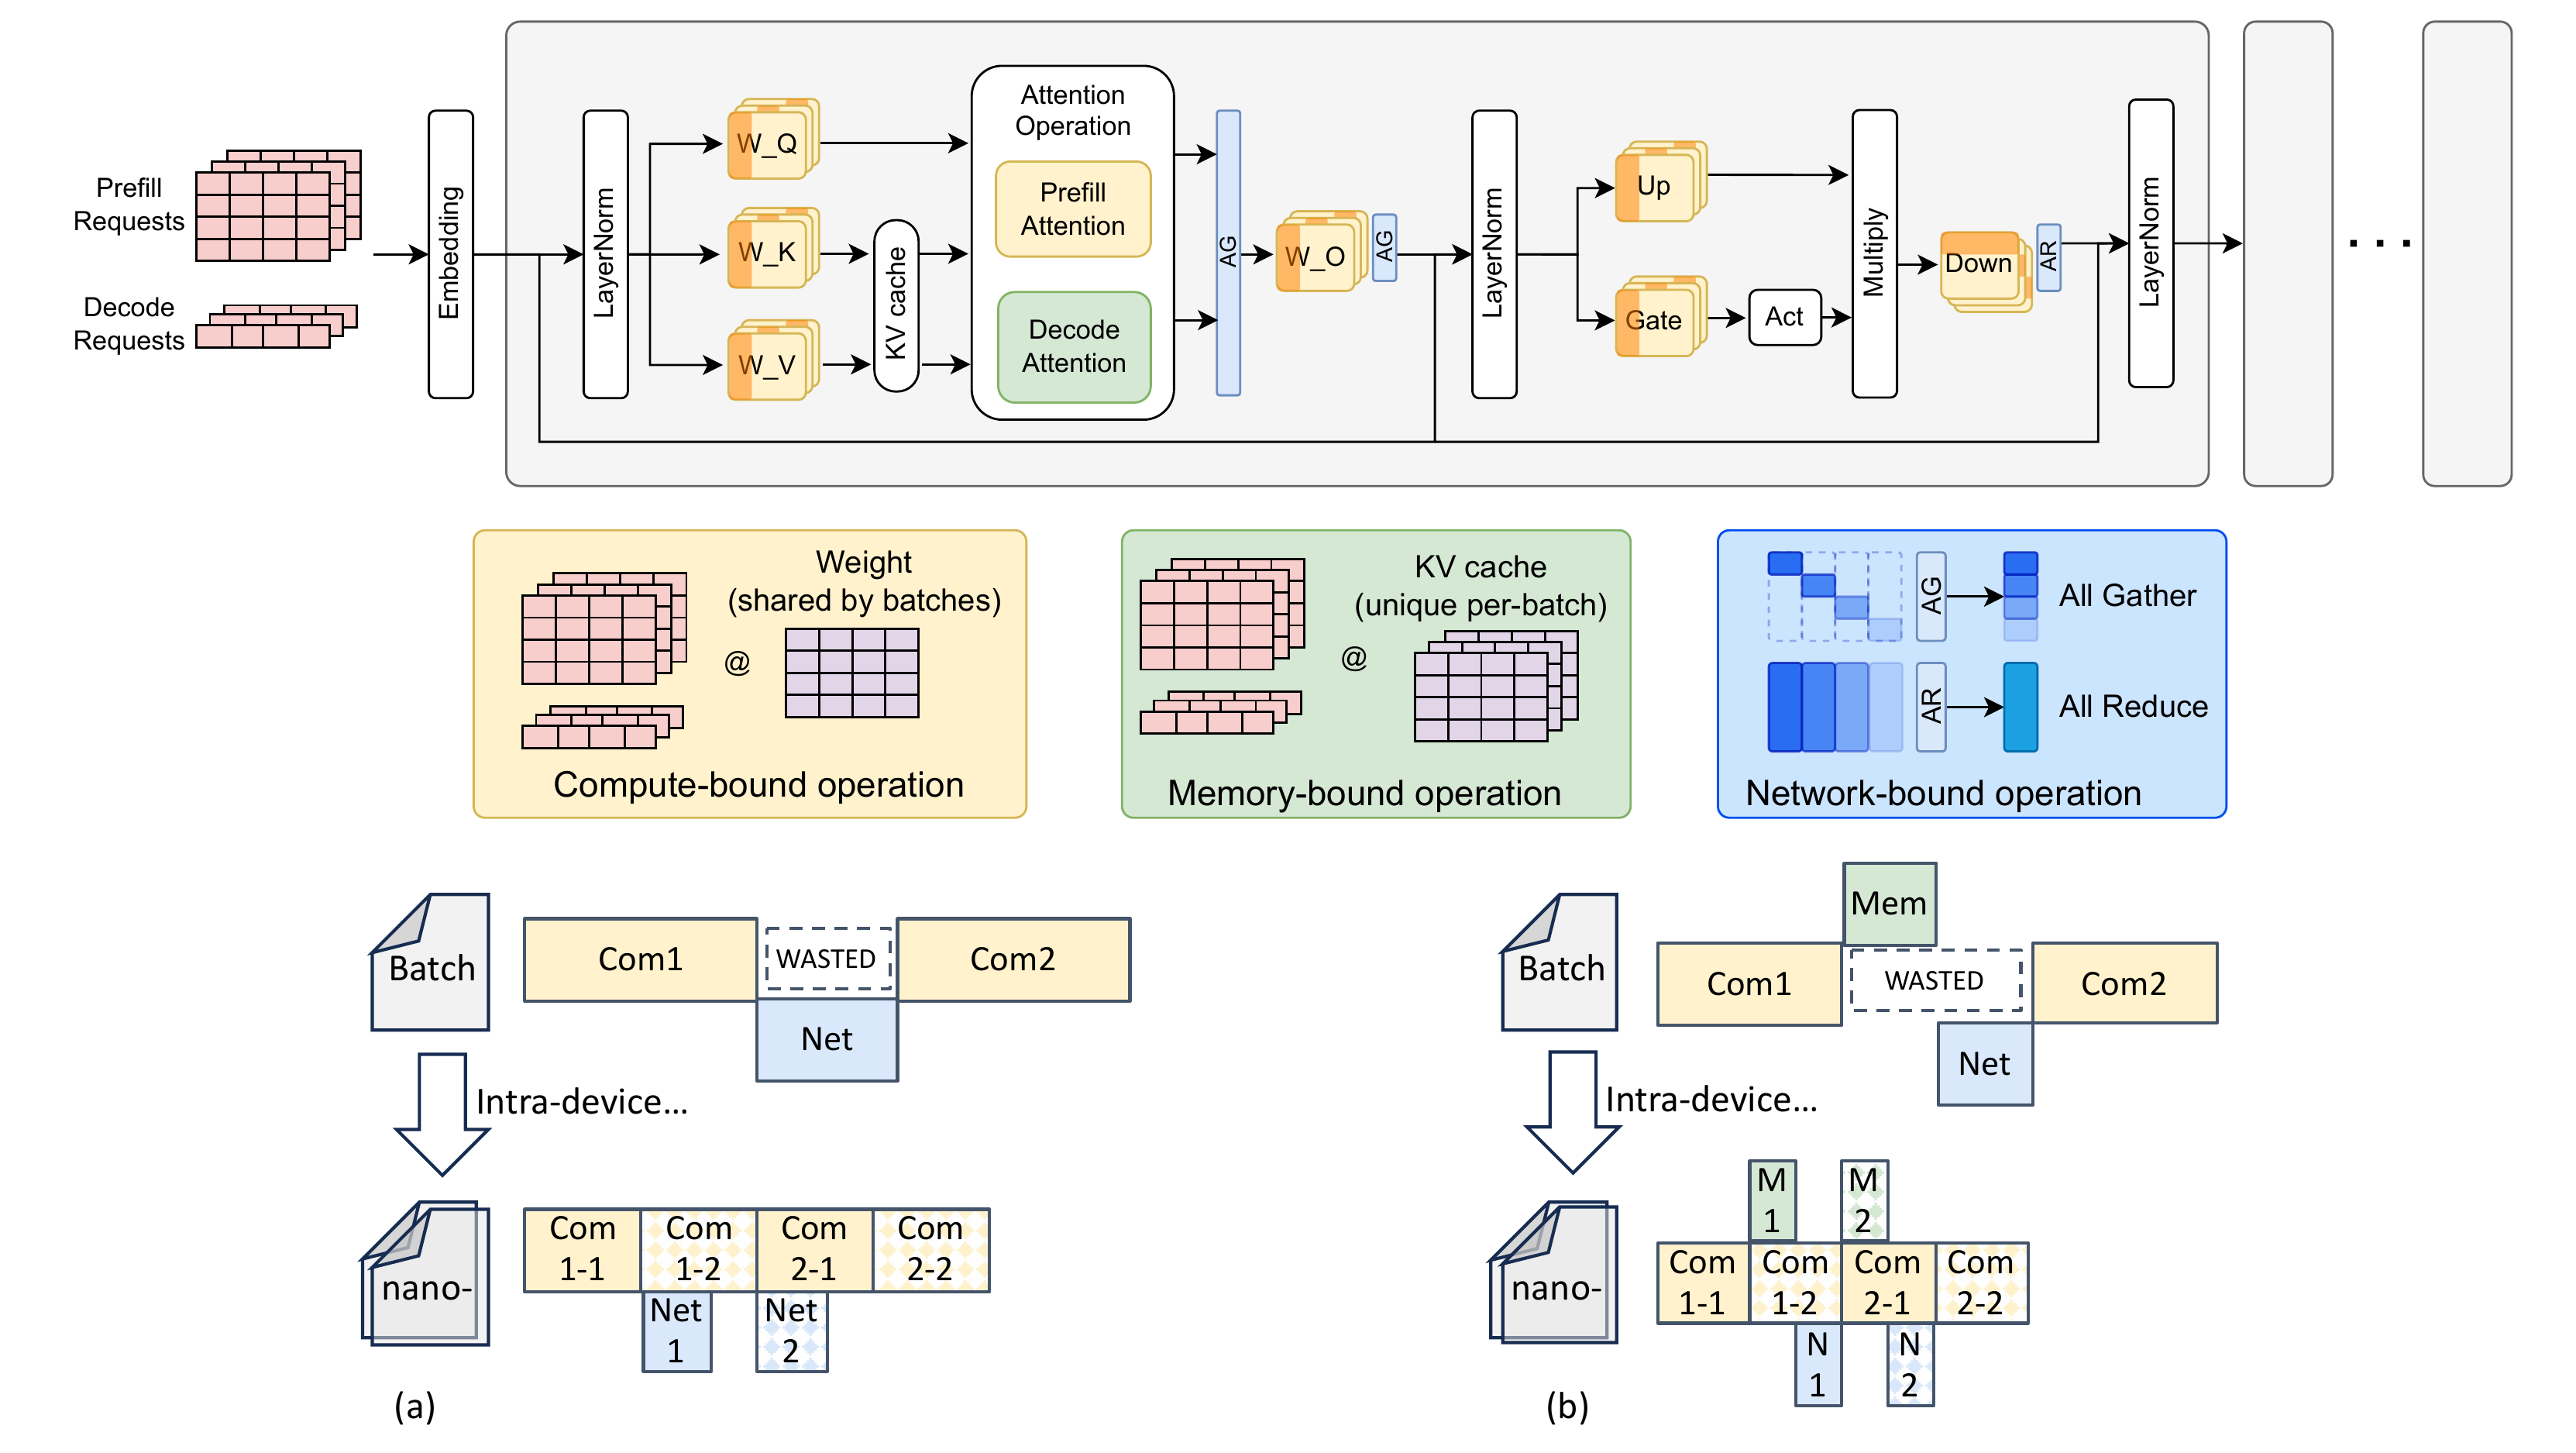
\includegraphics[width=\linewidth]{fig1_transformer.png}
  \caption{Transformer architecture, reproduced from the original paper. ...}
  \label{fig:transformer}
\end{figure}
\end{lstlisting}

Line by line:

\begin{itemize}[leftmargin=*]
  \item \verb|\begin{figure}[t]| starts a figure. The \verb|[t]| is a
        \emph{placement hint} meaning ``try to put this at the \textbf{t}op of a
        page.'' LaTeX treats figures as ``floats'' --- it slides them to a tidy
        spot near the text rather than locking them exactly in place.
  \item \verb|\centering| centers the image horizontally.
  \item \verb|\includegraphics[width=\linewidth]{...}| inserts the image file and
        scales it so its \verb|width| equals \verb|\linewidth| (the full text
        width). The filename is found via the \verb|figures/| path set earlier.
  \item \verb|\caption{...}| is the caption printed under the figure; LaTeX adds
        the ``Figure 1'' label automatically.
  \item \verb|\label{fig:transformer}| lets \verb|\ref| refer to it by number.
\end{itemize}

You will also see \verb|\begin{figure*}| (with a star). The star version spans the
\emph{full page width} --- used for the wide pipeline diagram.

% ======================================================================
\section{Tables}

Tables are the most detailed part of your file. Here is a small version of the
pattern:

\begin{lstlisting}
\begin{table}[t]
\centering
\caption{The average and standard deviation of input and output lengths ...}
\label{tab:datasets}
\begin{tabular}{lrr}
\toprule
\textbf{Dataset} & \textbf{Avg. Input (Std)} & \textbf{Avg. Output (Std)} \\
\midrule
Splitwise~\cite{patel2023splitwise}  & 1155 (1109) & 211 (163) \\
LMSYS-Chat~\cite{zheng2023lmsys}     & 102 (169)   & 222 (210) \\
\bottomrule
\end{tabular}
\end{table}
\end{lstlisting}

Two environments are nested here. The outer \verb|table| behaves like a figure (it
floats, has a \verb|\caption| and \verb|\label|). The inner \verb|tabular| holds
the actual grid. The key rules:

\begin{itemize}[leftmargin=*]
  \item \verb|{lrr}| defines the columns: here three columns, one
        \textbf{l}eft-aligned and two \textbf{r}ight-aligned. (\verb|c| would be
        centered.) So \verb|{llrrrrrrrr}| in your big table means ten columns with
        those alignments.
  \item Inside a row, \verb|&| \textbf{separates columns} and \verb|\\| \textbf{ends
        the row}.
  \item \verb|\toprule|, \verb|\midrule|, \verb|\bottomrule| (from the
        \verb|booktabs| package) draw the clean horizontal lines at the top, under
        the header, and at the bottom.
\end{itemize}

A few extras that appear in your larger tables:

\begin{itemize}[leftmargin=*]
  \item \verb|\multicolumn{7}{c}{...}| merges 7 columns into one centered cell
        (used for a header that spans several columns).
  \item \verb|\multirow{2}{*}{...}| merges a cell down across 2 rows.
  \item \verb|\cmidrule(lr){2-8}| draws a partial line under only columns 2--8.
  \item \verb|\setlength{\tabcolsep}{4pt}| reduces the space between columns so a
        wide table fits.
  \item \verb|\begin{table*}| (star) again means ``span the full page width,''
        used for the big accelerator table.
  \item Numbers like \verb|1{,}555| use \verb|{,}| so the comma is spaced as a
        thousands separator.
\end{itemize}

% ======================================================================
\section{The algorithm block}

\begin{lstlisting}
\begin{algorithm}[t]
\caption{\nf: Auto-search and Runtime Execution}
\label{alg:nanoflow}
\begin{algorithmic}[1]
\Require Model architecture $\mathcal{M}$, hardware spec $\mathcal{H}$, ...
\Ensure  Optimized intra-device pipeline $\Pi$, ...
\State $\Bdense \gets \Call{MaxDenseBatch}{...}$ \Comment{largest batch ...}
\ForAll{$k \in \{\text{GEMM}, \text{GEMV}, \text{Network}\}$}
  \State ...
\EndFor
\end{algorithmic}
\end{algorithm}
\end{lstlisting}

Again two nested environments: the outer \verb|algorithm| is a float (like a
figure, with caption ``Algorithm 1'' and a label), and the inner
\verb|algorithmic| holds the pseudocode. The \verb|[1]| makes it number the lines.
The pseudocode commands come from the \verb|algpseudocode| package:

\begin{itemize}[leftmargin=*]
  \item \verb|\State| --- one ordinary step/line.
  \item \verb|\Require| / \verb|\Ensure| --- the ``input'' and ``output''
        preconditions at the top.
  \item \verb|\For|, \verb|\ForAll|, \verb|\EndFor| --- a loop and its end.
  \item \verb|\If|, \verb|\EndIf|, \verb|\While|, \verb|\Repeat|, \verb|\Until| ---
        other control structures.
  \item \verb|\State $x \gets y$| --- the \verb|\gets| prints a left arrow
        ($\leftarrow$), meaning ``assign''.
  \item \verb|\Call{Name}{args}| --- formats a function call.
  \item \verb|\Comment{...}| --- a right-aligned comment on that line.
  \item \verb|\Statex| --- a line with no number (used for the ``Phase 0/1/2''
        headers).
\end{itemize}

The \verb|$\mathcal{M}$| style prints fancy calligraphic capitals used for the
model/hardware/workload sets.

% ======================================================================
\section{The bibliography (references)}

At the very end of the file:

\begin{lstlisting}
\bibliographystyle{ACM-Reference-Format}
\bibliography{references}
\end{lstlisting}

\begin{itemize}[leftmargin=*]
  \item \verb|\bibliography{references}| pulls in your \verb|references.bib| file
        (the ``.bib'' is assumed). That \verb|.bib| file is a database of sources,
        each with a key (like \verb|kwon2023efficient|), a title, authors, year,
        etc.
  \item \verb|\bibliographystyle{ACM-Reference-Format}| chooses \emph{how} the
        references are formatted --- here in the official ACM style your
        assignment asked for.
  \item Only sources you actually \verb|\cite| show up in the final list, and they
        are numbered/ordered automatically. This is why we never had to touch the
        \verb|.bib| file when removing figures: the citations in the text are what
        matter.
\end{itemize}

% ======================================================================
\section{The three fixes we made (in case your teacher asks)}
\label{sec:fixes}

When you first tried to compile, three real errors came up. Here is what they were
and the one-line fix for each:

\begin{enumerate}[leftmargin=*]
  \item \textbf{``\texttt{\textbackslash Bbbk} already defined.''} The \verb|acmart|
        style and the \verb|amssymb| package both try to define the same symbol.
        The fix, \verb|\let\Bbbk\relax| placed just before
        \verb|\usepackage{amssymb}|, temporarily ``clears'' that symbol so
        \verb|amssymb| can define it without complaint.
  \item \textbf{``Undefined control sequence \texttt{\textbackslash nf}.''} Your
        \verb|\nf| shortcut uses \verb|\xspace|, but the \verb|xspace| package was
        not loaded. Adding \verb|\usepackage{xspace}| fixed it.
  \item \textbf{``No country present for an affiliation.''} The \verb|acmart| class
        requires every author to have a \verb|\country{...}|. They were empty, so
        we filled in \verb|\country{USA}|.
\end{enumerate}

\vspace{4mm}
\hrule
\vspace{3mm}
\textbf{One-line summary you can give your teacher:} the file uses the required
\verb|acmart| document class, loads a handful of standard packages (graphics,
math, tables, algorithms), defines a couple of custom shortcuts, builds the title
block, and then writes the content using sections, figures, tables, equations, an
algorithm, and citations --- all of which LaTeX numbers and cross-references
automatically.

\end{document}
